\documentclass[10pt]{article}
\usepackage[margin=1in]{geometry}
\usepackage[T1]{fontenc}
\usepackage{booktabs}
\usepackage{amsmath}
\usepackage{amssymb}
\usepackage{graphicx}
\usepackage{xcolor}
\usepackage[colorlinks=true,allcolors=blue]{hyperref}
\usepackage{natbib}
\usepackage{microtype}
\usepackage{pgfplots}
\pgfplotsset{compat=1.18}
% Zwei kategoriale Slots, CVD-validiert (worst adjacent Delta-E 24.7 protan).
% Zusaetzlich Linienstil + Markerform, damit die Abbildung in Graustufen traegt.
\definecolor{sermoving}{HTML}{2A78D6}
\definecolor{serfrozen}{HTML}{EB6834}

\newcommand{\ptrue}{P(\textsc{True})}
\setlength{\parskip}{0.02em}

\title{What Does a Correctness Probe Measure?\\
\large Probing Position, Incremental Value, and the Operationalization\\
Sensitivity of Conflict-Subset Evaluation}

\author{Richard Eberle\\ resonaticAI \\ \texttt{richi@resonatic.ch}}
\date{\today}

\begin{document}
\maketitle

\begin{abstract}
Linear probes on hidden states predict whether a language model's answer is correct, and they
outperform simply asking the model. We do not dispute that---it has been established since
\citet{azaria2023internal}. We ask what such a probe measures, and report three findings.
\textbf{(1)~The probing position determines what the probe tracks, and the reported AUROC does not
reveal it.} At the last token of the yes/no self-verification prompt the probe's scores correlate
$0.91$--$0.99$ with the model's own yes/no logit margin and order correctness \emph{inversely} on
the conflict subset; at the answer position the same probe design tracks correctness. Aggregate
AUROC is nearly the same either way ($\approx0.73$--$0.87$).
\textbf{(2)~The probe carries decision-relevant information beyond what the model states.} In a
nested comparison on \emph{all} items---no subset selection---adding the probe to $\ptrue{}$
improves held-out log loss in 15/15 model $\times$ task cells ($+0.043$ to $+0.203$, all 90\%
intervals excluding zero).
\textbf{(3)~Conflict-subset conclusions are operationalization-sensitive.} The self-judgement
instrument jointly defines the construct and the evaluated population, so each wording measures a
different conditional estimand. Holding probe, data and labels fixed and substituting one of four
self-judgement instruments moves conflict AUROC by up to $0.279$ and, for one model, moves the
qualitative verdict across its decision boundary. We do \emph{not} claim published conclusions
reverse: under the high-confidence criterion actually used by \citet{diagnosing2026}, the conflict
cells degenerate on our base models and the comparison is not testable here.
Experiments span 5 models across 3 families, $n=6000$ questions. Three of our own claims were
retracted along the way; we report them in the main text, because they instantiate the thesis.
\end{abstract}

\section{Introduction}

Probes on hidden states are used to decide when to trust a model: to abstain, to escalate, to route
to a larger system. Whether such a probe reads \emph{correctness} or the model's \emph{opinion about
its correctness} changes what it is good for. A probe that recovers the model's opinion adds nothing
beyond asking; a probe that recovers correctness where the opinion is wrong is what selective
prediction needs.

Separating the two is hard because the labels agree on most items. The established approach is to
evaluate where they disagree \citep{diagnosing2026,masked2026}. We use that lever to establish a
positive result about probing position (Section~\ref{sec:position}), and then show that the lever is
sensitive to how the self-judgement instrument is worded (Section~\ref{sec:conflict}): because the
instrument defines both the construct and the evaluated population, each wording estimates a
different conditional quantity. This is a form of spectrum effect
\citep{ransohoff1978spectrum,hernan2004selection} rather than a flaw in any particular study.

Because of that sensitivity we also report the question that needs no subset at all
(Section~\ref{sec:incremental}): does the probe add decision-relevant information over what the
model already states? It does, in every cell we measured.

We arrived here by failing. We first reported a condition governing when probes collapse onto
self-judgement, then an intervention that appeared to confirm it causally. On inspection the probe
was byte-identical across all conditions; only the evaluation subset had moved. We report the
failure because the correction \emph{is} the contribution, and because a paper about measurement
discipline that hid its own errors would be self-refuting.

\section{Related work}

\citet{kadavath2022} introduce $\ptrue{}$ and P(IK) and show calibration improves with scale; we
reproduce this on Qwen3. \citet{azaria2023internal} show a hidden-state probe substantially
outperforms few-shot prompting, and that sequence probability tracks length and word frequency
rather than truth. \citet{orgad2024llms} is the canonical treatment of error signals in internal
representations. Work on linear ``truth'' directions \citep{burns2023discovering,marks2024geometry}
asks a related identification question from the unsupervised side. \textbf{We claim no novelty for
``probe beats prompting.''} Section~\ref{sec:f1} reports it only to show the distinction has
practical consequences.

\citet{diagnosing2026} factorises the correct/incorrect contrast into objective correctness (OC) and
self-judgement (SJ), giving cells A (correct/endorsed), B (correct/rejected), C
(incorrect/endorsed), D (incorrect/rejected), and finds that the transferable readout direction
follows SJ. Two details matter for our Section~\ref{sec:conflict}. That paper \emph{does} report its
judgement prompt verbatim (``Do you believe the answer above is correct? Answer only with Yes or
No.''); it uses a symmetric high-confidence criterion ($p \le 0.3$ or $p \ge 0.7$) rather than a
median split, discarding the ambiguous middle; and it complements the conflict analysis with an
all-cell fixed-effects model. What it does not do---and what we contribute---is evaluate whether the
semantic verdict is stable under alternative judgement formulations.

\citet{masked2026} compare self- against peer-model probes, finding an advantage for the
self-representation only on disagreement subsets and only for factual knowledge. Their subset is
defined by \emph{two models disagreeing on correctness labels} rather than by a prompted
self-judgement. Our result therefore does not bear on their construct, and we do not claim it
does.

Selective prediction and calibration provide the decision framing we adopt in
Section~\ref{sec:incremental} \citep{geifman2017selective,guo2017calibration}.

\section{Setup}
\label{sec:setup}

\paragraph{Models and data.} Qwen3-4B, Qwen3-8B, Qwen3.6-35B-A3B, Mistral-7B-v0.3, OLMo-2-7B; base
models, no instruction tuning, no adapters. $n=6000$ questions drawn with a fixed seed from PopQA
\citep{mallen2023popqa}, TriviaQA \citep{joshi2017triviaqa} and WebQuestions
\citep{berant2013webq}; identical items across models. Answers are produced by raw continuation
without a chat template with 5 fixed few-shot exemplars, and scored per dataset (PopQA substring
match; TriviaQA/WebQuestions normalised exact match).

\paragraph{$\ptrue{}$.} The model is asked, in a separate forward pass, whether its own answer is
correct. We read the logits at the final position and define
$\ptrue{} = \frac{\sum_{v \in \mathcal{Y}} p(v)}{\sum_{v \in \mathcal{Y}} p(v) + \sum_{v \in \mathcal{N}} p(v)}$
where $\mathcal{Y}$ and $\mathcal{N}$ are first-token ids for
\{\texttt{Ja}, \texttt{Yes}, \texttt{ja}, \texttt{yes}, \texttt{True}, \texttt{true}\} and the
corresponding negatives. Normalising over the two token sets rather than the full vocabulary makes
the quantity robust to tokenizer differences across families.

\paragraph{Probe.} Given hidden states $h_i \in \mathbb{R}^d$ and correctness labels
$y_i \in \{0,1\}$, the difference-of-means probe standardises per dimension using training
statistics and scores by $s_i = \tilde h_i \cdot w$ with
$w = \mathrm{mean}_{i \in \mathcal{C}} \tilde h_i - \mathrm{mean}_{i \in \mathcal{I}} \tilde h_i$
over correct and incorrect training items. There is no gradient training and no hyperparameter
beyond the layer.

\paragraph{From scores to probabilities.} The probe returns an unbounded score, not a probability.
Where a probability is needed we map scores through a one-dimensional logistic (Platt) fit on
training data only, with standardised inputs; $\ptrue{}$ enters as $\operatorname{logit}\ptrue{}$.
This matters for the fairness of Section~\ref{sec:incremental}: the baseline there is itself such a
fit, $Y \sim \sigma(a \operatorname{logit}\ptrue{} + b)$, so $\ptrue{}$ is recalibrated exactly as
the extended model is and the reported gain cannot be obtained by recalibration alone. The utility
threshold $p^\ast = \lambda/(1{+}\lambda)$ is applied to Platt-mapped probabilities, since it is
optimal only for calibrated ones. AUROC and $F_1$ require no probability---they depend on the
ranking and on one threshold---and use raw scores.

\paragraph{Splitting.} Two distinct procedures, kept separate throughout.
\emph{(i)~Probe scores} are out-of-fold: within each task, 5-fold cross-validation, scores
standardised per fold, averaged over 5 seeds; every item is scored by a probe that never saw it, so
all $n$ items are usable as test items. Probes are always fitted within a task.
\emph{(ii)~Downstream fitting}---classification thresholds (Section~\ref{sec:f1}) and combination
weights (Section~\ref{sec:incremental})---uses repeated random 50/50 splits over those out-of-fold
scores, 20 and 10 respectively, fitted on train and evaluated on held-out data.

\paragraph{How the threshold is chosen.} For $F_1$ we scan the training half for the
$F_1$-maximising cut---candidates are the distinct training scores, sub-sampled to 400 quantiles
when there are more---and apply the argmax unchanged to the held-out half. \textbf{The identical
procedure is applied to both signals}, so $\ptrue{}$ is not held to its nominal $0.5$, which would
be disastrous for Mistral ($96\%$ of items exceed it). Where $\ptrue{}$ fails in
Table~\ref{tab:f1} it fails at \emph{every} cut---the train-selected threshold degenerates to
``always yes''---which is what an AUROC near chance means. AUROC selects no threshold at all;
we report it alongside a fixed-threshold and a decision-theoretic view rather than on its own.

\paragraph{Positions and layers.} Hidden states are taken at 25/50/75/100\% of depth in a single
forward pass, at the last generated answer token, as returned by
\texttt{output\_\allowbreak hidden\_\allowbreak states}. We verified that only the final entry
of that tuple has the model's final normalisation applied; the intermediate depths we probe are raw
residual-stream states. We report 50\% as the main setting;
the sweep is in Appendix~\ref{app:sweep}. The contrasting position is the last token of the yes/no
prompt at the final layer.

\paragraph{Conflict subset.} Following \citet{diagnosing2026}, an item is in conflict if it is
correct while the model is unsure, or incorrect while the model is sure. Our main analysis uses a
per-task median split; a fixed absolute threshold is not comparable across models, since
$\ptrue{} > 0.5$ holds for 96\% of Mistral's items and 1\% of OLMo's. Section~\ref{sec:conflict}
also reports the high-confidence criterion of \citet{diagnosing2026}.

\section{The distinction has practical consequences}
\label{sec:f1}

\begin{table}[t]
\centering\footnotesize
\setlength{\tabcolsep}{4.5pt}
\begin{tabular}{lrrrrrrrrr}
\toprule
& \multicolumn{3}{c}{PopQA} & \multicolumn{3}{c}{TriviaQA} & \multicolumn{3}{c}{WebQuestions} \\
\cmidrule(lr){2-4}\cmidrule(lr){5-7}\cmidrule(lr){8-10}
Model & $\ptrue{}$ & Probe & always & $\ptrue{}$ & Probe & always & $\ptrue{}$ & Probe & always \\
\midrule
Qwen3-4B    & 0.590 & 0.591 & 0.312 & 0.712 & 0.745 & 0.603 & 0.459 & 0.524 & 0.334 \\
Qwen3-8B    & 0.601 & 0.624 & 0.376 & 0.790 & 0.787 & 0.727 & 0.465 & 0.565 & 0.422 \\
Qwen3.6-35B & 0.609 & 0.619 & 0.485 & 0.788 & 0.861 & 0.739 & 0.468 & 0.597 & 0.407 \\
Mistral-7B  & \textbf{0.504} & 0.636 & \textbf{0.502} & \textbf{0.818} & 0.833 & \textbf{0.818} & \textbf{0.452} & 0.587 & \textbf{0.439} \\
OLMo-2-7B   & 0.559 & 0.623 & 0.494 & \textbf{0.812} & 0.845 & \textbf{0.813} & \textbf{0.795} & 0.819 & \textbf{0.796} \\
\bottomrule
\end{tabular}
\caption{$F_1$ with the threshold chosen on training data, evaluated held-out, 20 splits;
``always'' is the trivial always-answer-yes baseline. The probe is higher in 14/15 cells; the
exception (Qwen3-8B/TriviaQA, $0.787$ vs $0.790$) and the smallest win (Qwen3-4B/PopQA, $+0.001$)
are both within resampling noise and we read neither as a difference. In the five boldface pairs
$\ptrue{}$ does not beat the trivial baseline (margin $\le 0.013$): recall exceeds $0.99$ and it
reproduces the base rate. \emph{This comparison is motivation, not contribution}
\citep{azaria2023internal,orgad2024llms}.}
\label{tab:f1}
\end{table}

Table~\ref{tab:f1} reports classification quality. What matters is not that the probe wins; it is
\emph{how} the prompted self-check fails. In a third of the cells it does not beat the trivial
baseline at any threshold---it answers ``yes, correct'' to nearly everything. The same degeneracy
appears under a selective-prediction utility ($+1$ correct, $-\lambda$ incorrect, $0$ abstain) with
the analytic threshold $p^\ast = \lambda/(1{+}\lambda)$: $\ptrue{}$ collapses to zero coverage in
34 of 75 model $\times$ task $\times$ $\lambda$ cells, and its AUROC falls to $0.430$ on
Mistral/PopQA, below chance, where the probe reaches $0.797$.

\section{Finding 1: the probing position determines what the probe tracks}
\label{sec:position}

\begin{table}[t]
\centering\footnotesize
\setlength{\tabcolsep}{4pt}
\begin{tabular}{lrrrrrrr}
\toprule
& \multicolumn{4}{c}{Yes/no-prompt position (final layer)} & \multicolumn{3}{c}{Answer position (mid-depth)} \\
\cmidrule(lr){2-5}\cmidrule(lr){6-8}
Model & $r(s,m)$ & $\rho$ & Conflict & All items & $\rho$ & Conflict & All items \\
\midrule
Qwen3-4B    & $0.98$--$0.99$ & $+0.98\ldots{+}0.99$ & $0.001$--$0.035$ & 0.73--0.85 & $+0.45\ldots{+}0.54$ & $0.593$--$0.687$ & 0.82--0.87 \\
Qwen3-8B    & $0.97$--$0.99$ & $+0.97\ldots{+}0.98$ & $0.002$--$0.008$ & 0.69--0.83 & $+0.35\ldots{+}0.63$ & $0.451$--$0.784$ & 0.78--0.88 \\
Qwen3.6-35B & $0.91$--$0.96$ & $+0.97\ldots{+}0.99$ & $0.011$--$0.033$ & 0.70--0.79 & $+0.36\ldots{+}0.46$ & $0.680$--$0.812$ & 0.80--0.89 \\
OLMo-2-7B   & $0.46$--$0.83$ & $-0.07\ldots{+}0.92$ & $0.115$--$0.652$ & 0.62--0.74 & $+0.04\ldots{+}0.66$ & $0.382$--$0.730$ & 0.74--0.80 \\
Mistral-7B  & $0.37$--$0.79$ & $-0.37\ldots{+}0.52$ & $0.478$--$0.867$ & 0.69--0.75 & $-0.33\ldots{+}0.26$ & $0.704$--$0.887$ & 0.78--0.80 \\
\bottomrule
\end{tabular}
\caption{Same data, same labels, same probe design; only the hidden-state position differs.
$r(s,m)$ is the correlation between the probe score and the model's own yes/no logit margin
$m = h^\top(u_{\text{yes}} - u_{\text{no}})$, read directly from the unembedding matrix; $\rho$ is
Spearman correlation between probe score and $\ptrue{}$; ``Conflict'' is probe AUROC against
correctness on $B \cup C$; ``All items'' is the ordinary aggregate. Ranges are over the three tasks.
For the three Qwen models the yes/no position gives a probe that is all but identical to the
self-judgement readout, while the aggregate AUROC barely separates the two positions.}
\label{tab:position}
\end{table}

At the last token of the yes/no prompt, the yes/no logit margin is
$m = h^\top(u_{\text{yes}} - u_{\text{no}})$, a linear function of the very state being probed
($u$ from the unembedding matrix; this is also the state the language-model head consumes, since
only the last entry of the hidden-state tuple carries the final normalisation). That position makes
the self-judgement \emph{directly linearly decodable}. It does not follow that a probe trained on
correctness labels must recover that direction---difference-of-means solves a different objective.
We therefore measured it: the correlation between probe score and the model's own yes/no margin is
$0.91$--$0.99$ in all nine Qwen cells (Table~\ref{tab:position}, column $r(s,m)$), falling to
$|r| \le 0.45$ at the answer position.

On the conflict subset those probes reach AUROC $0.001$--$0.036$. This is not an absence of signal:
an AUROC near zero is a near-perfect \emph{inverse} ordering of correctness, which is exactly what a
copy of the self-judgement produces on a subset defined as ``where the self-judgement is wrong.''
Moving the probe to the answer position---where no self-verification prompt is in context, as in
\citet{azaria2023internal} and \citet{orgad2024llms}---restores correctness tracking.

\paragraph{The reported metric does not distinguish the two.} Aggregate AUROC is $0.73$--$0.85$ at
the collapsed position and $0.82$--$0.87$ at the informative one. A reader given only that number
cannot tell which probe they have. Probing position is rarely reported.

\paragraph{Not affected by Section~\ref{sec:conflict}.} Both positions share the same $\ptrue{}$ and
therefore the same conflict subset by construction; cell sizes are identical row-wise (Qwen3-8B/
PopQA: $B{=}87$, $C{=}595$ at both positions). The sensitivity we describe below arises only when
$\ptrue{}$ itself changes.

\paragraph{The exceptions follow the same measure.} The collapse is not universal: Mistral shows
none at the yes/no position on PopQA, and OLMo collapses on two of three tasks. The alignment
measure accounts for this. Ordering all 15 cells by $r(s,m)$ at the yes/no position puts the nine
Qwen cells on top ($0.91$--$0.99$) and the three non-collapsing cells at the bottom---Mistral/WebQ
$0.37$, Mistral/PopQA $0.43$, OLMo/WebQ $0.46$. Across the 15 cells, Spearman correlation between
$r(s,m)$ and $\rho$ is $+0.71$; both quantities are subset-free, so this relation is not exposed to
the sensitivity of Section~\ref{sec:conflict}. Where the self-judgement direction is strongly
present in the probed state, the correctness-labelled probe recovers it; where it is not, the probe
does not collapse. We earlier proposed $\ptrue{}$ \emph{strength} as the governing quantity and
retracted it (Section~\ref{sec:retractions}); the alignment of the probed state with the readout
direction is the better-behaved candidate, and it is measured rather than inferred.

\section{Finding 2: the probe adds decision-relevant information over $\ptrue{}$}
\label{sec:incremental}

\begin{table}[t]
\centering\small
\begin{tabular}{lrrrrr}
\toprule
Model & $\Delta$ log loss (PopQA / TriviaQA / WebQ) & \multicolumn{3}{c}{$\Delta$ AUROC} & $w_{\text{probe}}$ \\
\midrule
Qwen3-4B    & $+0.065$ \; / \; $+0.104$ \; / \; $+0.072$ & $+0.071$ & $+0.078$ & $+0.118$ & $1.30$--$1.37$ \\
Qwen3-8B    & $+0.100$ \; / \; $+0.061$ \; / \; $+0.080$ & $+0.103$ & $+0.041$ & $+0.129$ & $1.09$--$1.45$ \\
Qwen3.6-35B & $+0.072$ \; / \; $+0.203$ \; / \; $+0.103$ & $+0.077$ & $+0.134$ & $+0.144$ & $1.01$--$2.09$ \\
Mistral-7B  & $+0.119$ \; / \; $+0.096$ \; / \; $+0.104$ & $+0.226$ & $+0.169$ & $+0.207$ & $1.14$--$1.26$ \\
OLMo-2-7B   & $+0.043$ \; / \; $+0.118$ \; / \; $+0.090$ & $+0.077$ & $+0.191$ & $+0.223$ & $1.00$--$1.33$ \\
\bottomrule
\end{tabular}
\caption{Nested comparison on \emph{all} items: logistic
$Y \sim \sigma(a \operatorname{logit}\ptrue{} + b)$ against
$Y \sim \sigma(a \operatorname{logit}\ptrue{} + c\,s_{\text{probe}} + b)$; both fitted on
train, evaluated held-out, 10 splits, paired bootstrap. The baseline is a recalibration of
$\ptrue{}$, so the gain is not a calibration artifact. Positive $\Delta$ favours the extended model. All 15 cells have 90\% intervals
strictly above zero for log loss (smallest lower bound $+0.024$); $\Delta$ Brier is
$+0.015$ to $+0.077$. No subset selection is involved.}
\label{tab:incremental}
\end{table}

Semantic identification through the conflict subset turns out to depend on how that subset is
constructed (Section~\ref{sec:conflict}). The decision-theoretic question does not require a subset
at all: given what the model already says about itself, does the probe add anything? We answer it as
a nested model comparison on all items, reported in Table~\ref{tab:incremental}.

It does, in 15 of 15 cells, on log loss, Brier score and AUROC simultaneously, with a probe weight
consistently near or above that of $\ptrue{}$ itself. This claim is weaker than ``the probe encodes
correctness''---it makes no assertion about what a latent direction represents---and correspondingly
harder to dispute. For a system that must decide whether to answer, abstain or escalate, it is also
the claim that matters.

\section{Finding 3: conflict-subset conclusions are operationalization-sensitive}
\label{sec:conflict}

The self-judgement instrument does two jobs at once: it defines the construct being compared
against, and it selects the population on which the comparison is evaluated. Conflict AUROC is
therefore not one quantity but a family, indexed by the instrument:
$\mathrm{AUROC}(s, Y \mid i \in B_j \cup C_j)$ for instrument $j$. Different wordings estimate
different conditional quantities, so they need not agree---a spectrum effect
\citep{ransohoff1978spectrum} rather than an error in any particular study.

We make the magnitude concrete with four self-judgement instruments that differ in language, chat
template and how sharply the correctness criterion is stated. This is deliberately not a
single-factor manipulation; it is four plausible instruments a practitioner might choose. Model,
items, generated answers, labels, hidden states and probe are all held fixed---possible because the
answer prompt contains no yes/no component, so answer-position states do not depend on the
self-evaluation wording at all.

\begin{figure}[t]
\centering
\pgfplotsset{
  every axis/.append style={
    width=\linewidth, height=4.6cm,
    ymin=0.32, ymax=0.99, ytick={0.4,0.5,0.6,0.7,0.8,0.9},
    xtick={1,2,3,4}, xmin=0.6, xmax=4.4,
    tick align=outside, tick style={semithick, black!45},
    axis line style={semithick, black!45},
    grid=major, grid style={very thin, black!12},
    label style={font=\footnotesize}, tick label style={font=\scriptsize},
    title style={font=\footnotesize\bfseries, yshift=-3pt},
    xlabel={self-judgement instrument (one point each)},
    xticklabel style={rotate=18, anchor=north east, xshift=3pt, font=\scriptsize},
  },
  moving/.style={sermoving, very thick, mark=*, mark size=2.2pt,
                 mark options={fill=sermoving, draw=white, line width=0.5pt}},
  frozen/.style={serfrozen, very thick, dashed, mark=square, mark size=2.4pt,
                 mark options={solid, draw=serfrozen, line width=0.9pt}},
}
\begin{minipage}{0.49\linewidth}
\begin{tikzpicture}
\begin{axis}[title={OLMo-2-7B, PopQA}, ylabel={Probe AUROC on conflict subset},
  xticklabels={``good?'', ``correct?''\,de, ``correct?''\,en, strict}]
  \addplot[moving] coordinates {(1,0.661) (2,0.382) (3,0.435) (4,0.415)};
  \addplot[frozen] coordinates {(1,0.382) (2,0.382) (3,0.382) (4,0.382)};
  \draw[black!45, thin, densely dotted] (axis cs:0.6,0.5) -- (axis cs:4.4,0.5);
  \node[anchor=west, font=\scriptsize, text=black!55] at (axis cs:1.9,0.545)
       {decision boundary};
\end{axis}
\end{tikzpicture}
\end{minipage}\hfill
\begin{minipage}{0.49\linewidth}
\begin{tikzpicture}
\begin{axis}[title={Mistral-7B-v0.3, PopQA}, ylabel={},
  xticklabels={``good?'', ``correct?''\,de, strict, ``correct?''\,en}]
  \addplot[moving] coordinates {(1,0.924) (2,0.887) (3,0.710) (4,0.670)};
  \addplot[frozen] coordinates {(1,0.887) (2,0.887) (3,0.887) (4,0.887)};
  \draw[black!45, thin, densely dotted] (axis cs:0.6,0.5) -- (axis cs:4.4,0.5);
\end{axis}
\end{tikzpicture}
\end{minipage}

\vspace{1pt}
\centering
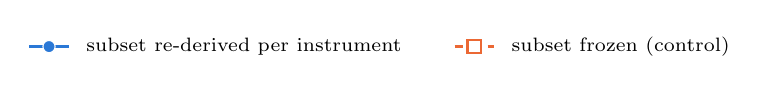
\begin{tikzpicture}
  \draw[sermoving, very thick] (0,0) -- (0.5,0);
  \filldraw[sermoving, draw=white, line width=0.4pt] (0.25,0) circle (2.2pt);
  \node[anchor=west, font=\scriptsize] at (0.6,0) {subset re-derived per instrument};
  \draw[serfrozen, very thick, dashed] (5.4,0) -- (5.9,0);
  \draw[serfrozen, line width=0.9pt, fill=white] (5.65,0) +(-2.4pt,-2.4pt) rectangle +(2.4pt,2.4pt);
  \node[anchor=west, font=\scriptsize] at (6.0,0) {subset frozen (control)};
\end{tikzpicture}
\caption{Each point is one self-judgement instrument (four per panel, ordered by the resulting
$\ptrue{}$ AUROC). The probe is \emph{identical} at every point: same hidden states, same labels,
same out-of-fold scores; probe AUROC over all items is constant at $0.795$ (OLMo) and $0.797$
(Mistral). Only the instrument changes, which changes which items enter the conflict subset.
Blue: subset re-derived per instrument, as in standard practice---the measured result moves by
$0.279$ (OLMo) and $0.254$ (Mistral), and for OLMo crosses the $0.5$ boundary that separates the
two qualitative verdicts. Orange: subset frozen from the baseline instrument---flat by construction
(see text).}
\label{fig:conflict}
\end{figure}

Figure~\ref{fig:conflict} shows the result. Asking ``Is this a good answer?'' rather than ``Is the
proposed answer correct?'' changes OLMo's conflict AUROC on PopQA from $0.382$ to $0.661$, moving it
across the boundary that separates ``the probe follows self-judgement'' from ``the probe follows
correctness.'' The probe was never retrained and its per-item scores are unchanged.

\paragraph{On the frozen control.} Deriving the subset once and substituting only $\ptrue{}$ leaves
conflict AUROC exactly constant. That is expected analytically---with probe, labels and evaluated
items all fixed, the statistic cannot move---and we report it as a consistency check, not as a
finding. The informative quantity is the $0.279$, not the $0.000$: it establishes that the entire
observed movement is attributable to population change rather than to anything about the probe.

\paragraph{We do not claim published conclusions reverse.} \citet{diagnosing2026} uses a
high-confidence criterion ($p \le 0.3$ or $p \ge 0.7$) rather than a median split, which discards
ambiguous items and is more robust to exactly this effect. Applying that criterion to our base
models leaves 23 of 24 model $\times$ task $\times$ instrument cells with a conflict cell below 25
items---Mistral has \emph{no} correct-and-rejected items at all, since its $\ptrue{}$ almost never
falls below $0.3$. On base models the high-confidence criterion is therefore not evaluable, and our
demonstration speaks to median-split operationalizations only. That restriction is itself worth
recording: an instrument that discards 70--95\% of items on base models is not a drop-in choice.

\paragraph{Why the movement happens.} When the instrument is more discriminative, the items on which
it errs are the harder ones. A subset selected by ``where the self-check is wrong'' is therefore not
a fixed population: sharpening the instrument enriches the subset for difficulty, and the probe
scores lower there for reasons unrelated to what it encodes.

\paragraph{Recommendation.} Report the judgement wording (as \citet{diagnosing2026} does), and
either freeze the subset definition across compared conditions or check the verdict under at least
one alternative instrument. Where possible, complement subset-conditional analysis with an
all-items estimand such as Section~\ref{sec:incremental}.

\section{What survives, and what we retracted}
\label{sec:retractions}

Across the 15 cells at the answer position, $\ptrue{}$ AUROC ranges from $0.430$ to $0.829$
($\mathrm{sd}=0.115$) while probe AUROC ranges from $0.736$ to $0.886$ ($\mathrm{sd}=0.039$): the
prompted self-check varies enormously, the probe is uniformly serviceable. Measured without the
conflict subset, Spearman correlation between $\ptrue{}$ strength and probe quality is $+0.74$---the
\emph{opposite} sign of what the conflict-subset metric suggests ($-0.41$). Both signals share a
difficulty driver, so we state this as correlational.

Three claims did not survive, all following the same pattern: an effect visible in a convenient
metric that vanishes in a clean one.
\textbf{(i)~``Asking is enough.''} A within-task null between probe and $\ptrue{}$ from an
underpowered design---a single split and two independent confidence intervals, when both signals
score the same items. Under a paired bootstrap on the difference with out-of-fold scores and TOST
against a $\pm0.05$ margin, the null reversed.
\textbf{(ii)~``OLMo's $\ptrue{}$ carries no signal.''} An artifact of an $n{=}385$ diagnostic run;
at $n{=}6000$ its AUROC is $0.717$ on PopQA.
\textbf{(iii)~A collapse condition and its apparent causal confirmation.} We reported that
$\ptrue{}$ strength governs whether a probe tracks correctness or self-judgement, then that a prompt
intervention confirmed it with Spearman $-1.00$ in three of three tasks. Both are artifacts of the
sensitivity analysed in Section~\ref{sec:conflict}: the probe was identical across conditions and
only the evaluated population moved.

\section{Implications for selective prediction and epistemic routing}

A control layer deciding when to answer, abstain or escalate should treat a probe as
context-dependent telemetry, not a truth oracle. A deployed probe needs a \emph{measurement
contract}: extraction position and layer, the task stratum it was fitted on, the judgement
instrument any comparison used, the calibration population, and the decision utility it is
thresholded for. Each changed a conclusion somewhere in this paper while leaving the reported
aggregate AUROC nearly untouched. Section~\ref{sec:incremental} is the evidence such a layer should
require before adding a signal: incremental decision value on the deployment population.

\section{Limitations}

Single machine. Bootstrap intervals quantify uncertainty given an item sample; re-extracting two
models with a fresh sample moves no cell between ``follows correctness'' and ``follows
self-judgement'' (12 cells, median $|\Delta|$ conflict AUROC $0.016$), though two Mistral cells
near $0.5$ cross the undecided band. The verifier is substring or normalised exact match, which rewards longer answers
\citep{azaria2023internal}. Out-of-fold scoring is transductive: an item's score comes from a probe
fitted on $4/5$ of the data, which excludes that item but includes others from the same downstream
evaluation half. No item's own label enters its own score; this is the price of using all $n$ items
as test items rather than a third of them. We probe one layer at one token position, so the probe
sees a contextual summary rather than the full activation tensor. We did vary the pooling axis:
mean-pooling over the answer tokens instead of taking the last one lowers probe AUROC in 14/15
cells---answers are 1--2 words, so averaging dilutes---but changes \emph{no} verdict (0/15), so the
last-token choice is not load-bearing for our conclusions. Our conflict analysis uses a median split; the high-confidence criterion
of \citet{diagnosing2026} is not evaluable on base models (Section~\ref{sec:conflict}), so we cannot
say whether the sensitivity persists there. The four instruments differ on several axes at once, so
we quantify instrument sensitivity, not the effect of any single factor. Prompt variation moves
$\ptrue{}$ calibration far more than its discrimination. The stability and alignment relations
(Sections~\ref{sec:position}, \ref{sec:retractions}) are correlational. We study short-form factual
QA only; \citet{masked2026} report a different pattern for mathematical reasoning.

\section{Conclusion}

A correctness probe's reported AUROC does not tell you what it measures. Position decides it---at the
self-verification position the probe is all but the model's own yes/no readout---and the standard
method for finding out estimates a different quantity for each judgement instrument, to the point of
moving a verdict across its decision boundary. Report probing position and judgement wording, freeze
the evaluated subset across compared conditions, and report incremental decision value on all items
alongside any subset-conditional claim. Our own strongest claim died to this sensitivity; we doubt
it is the only one.

\section*{Reproducibility}

All experiments ran on a single machine. Code, run scripts and the cached model outputs behind
every table are at \url{https://github.com/ResonaticAI-GmbH/what-probes-measure}: Tables~\ref{tab:f1}
and~\ref{tab:incremental} recompute on CPU in minutes from the included caches; analyses needing
hidden-state dumps ($\approx 2.2$\,GB) require one GPU extraction pass, scripted.

\appendix
\section{Layer sweep}
\label{app:sweep}

Probing at 25/50/75/100\% of depth at the answer position. The conflict-test verdict is stable
across depth (13 of 15 cells ``follows correctness'' at three of four depths); mean probe AUROC is
$0.743$, $0.815$, $0.794$, $0.787$. Choosing the shallowest depth instead lowers $\rho$ with
$\ptrue{}$ for the Qwen models ($0.22$--$0.32$ against $0.40$--$0.49$) but not for Mistral or OLMo
($+0.03$, $+0.06$), and costs $0.072$ AUROC on average. We selected mid-depth on the
pre-registerable ground of ``middle of the network'' rather than by outcome.

\section{Euclidean cosine is the wrong similarity here}
\label{app:cosine}

The natural direction-level test---cosine between the probe direction $w/\sigma$ and
$u_{\text{yes}} - u_{\text{no}}$---is uninformative in these representations: at the yes/no position
it gives $0.001$--$0.20$ across models against a random floor of $1/\sqrt{d} \approx 0.02$, with a
label-permutation control of comparable size. What matters is the alignment of the \emph{projections}
on the data, $\operatorname{corr}(h^\top w_1, h^\top w_2) = w_1^\top \Sigma w_2 /
\sqrt{w_1^\top \Sigma w_1 \cdot w_2^\top \Sigma w_2}$, and LLM hidden states are strongly
anisotropic: two directions can be nearly orthogonal yet produce near-identical projections. We
therefore report $r(s,m)$, which is the quantity the claim is about.

\section{Pooling across tasks}
\label{app:pooling}

Averaging over tasks with different base rates makes AUROC report a mixture of within-task
discrimination and between-task separation. On our three QA datasets the effect is modest and
\emph{negative} for the probe: pooled minus mean within-task AUROC is $-0.015$ to $-0.039$. In an
earlier configuration including GSM8K and SVAMP, where base rates diverge far more sharply, the same
comparison gave aggregate $0.89$--$0.95$ against within-task $0.67$--$0.86$; that configuration was
not re-run under the present protocol. Direction and magnitude depend on the task mix, so we report
within-task numbers throughout.

{\footnotesize
\setlength{\bibsep}{0pt plus 0.1ex}
\bibliographystyle{abbrvnat}
\bibliography{refs}
}
\end{document}
